\documentclass[ULlof]{ULrapport}

% Chargement des packages
\usepackage[utf8]{inputenc}
\usepackage[autolanguage]{numprint}
\usepackage{icomma}
\usepackage{multirow}
\usepackage{tabularx}
\usepackage{pbox}
\usepackage{float}
\usepackage{pifont}
\usepackage{Listings}
\usepackage{color}
\usepackage{graphicx}
%\usepackage{pdfpages} Package introuvable

\setcounter{tocdepth}{2}

% Page titre
\TitreProjet{Visualiseur interactif de scènes 3D}
\TitreRapport{Document de design -- Remise TP2}
\Destinataire{Philippe Voyer}
\NomEquipe{Équipe 4}
\TableauMembres{
   111\,127\,868  & Jérémie Bolduc & \\\hline
<<<<<<< HEAD
   111\,xxx\,xxx  & Gabriel Chantal & \\\hline
   111\,152\,662  & Alex Gilbert & \\\hline
=======
   111\,126\,561  & Gabriel Chantal & \\\hline
   111\,xxx\,xxx  & Alex Gilbert & \\\hline
>>>>>>> 9e08ca082e00dbe2a20f7b248cb4229f7a1200de
   111\,130\,693  & Alexandre McCune & \\\hline
   111\,xxx\,xxx  & Tania Toloza & \\\hline
}
\DateRemise{12 mars 2017}


\HistoriqueVersions{
   1.0 & 16 février 2017 & Création du document \\\hline
}

\definecolor{dkgreen}{rgb}{0,0.6,0}
\definecolor{gray}{rgb}{0.5,0.5,0.5}
\definecolor{mauve}{rgb}{0.58,0,0.82}

\lstset{frame=tb,
	language=C++,
	aboveskip=3mm,
	belowskip=3mm,
	showstringspaces=false,
	columns=flexible,
	basicstyle={\small\ttfamily},
	numbers=none,
	numberstyle=\tiny\color{gray},
	keywordstyle=\color{blue},
	commentstyle=\color{dkgreen},
	stringstyle=\color{mauve},
	breaklines=true,
	breakatwhitespace=true,
	tabsize=3
}

\begin{document}
	
\chapter{Sommaire}
\label{s:sommaire}

Cette application permet de construire, éditer et rendre des scènes 3D.  Notre équipe à développer plusieurs fonctionnalités en lien avec le traitement d’image, le dessin vectoriel, les transformations géométriques, la géométrie et le concept de caméra. 
Ce projet vise à développer un visualiseur interactif basé sur les notions de l’infographie. Nous avons, donc implémenté des fonctionnalités qui permettent à l’utilisateur de construire des scènes avec différentes entités géométriques.  Des entités tels que des cubes, triangles, lignes, points, cercle et des carrés peuvent être construit selon des paramètres choisi par l’utilisateur. 
L’utilisateur peut construire des scènes interactivement et exporter des images. 
Dans ce document, les différentes fonctionnalités seront détaillées et des parties du code seront présentés.  Un diagramme présentera l’ensemble des fonctions de l’application.  De cette façon, une vue d’ensemble pourra bien d’écrire l’architecture de l’application
Nous présentons également les technologies que nous avons utilisé pour développer le visualiseur interactif de scène 3D. 
 

\chapter{Interactivité}
\label{s:interactivite}

L’option Dessiner Primitive permet d’ajouter une primitive dans la scène. L’utilisateur peut choisir les valeurs pour la couleur du fond de la scène. 
L’application permet d’importer des modèles et de les représenter en 3D. Il est aussi possible d’exporter à l’aide de l’option Exportation en image. 
L’option Type permet à l’utilisateur de choisir le type de primitive voulu soit en 2D, soit en 3D. 
Pour les primitives en 3D il est possible de choisir la position en X, Y et Z. La taille est définie par la hauteur, largeur et profondeur.
Pour les primitives en 2D il est possible de choisir la position en X et Y.  La taille est définie par la hauteur et largeur.
L’utilisateur peut également modifier la couleur de remplissage des primitives choisi, la couleur de la bordure et l’épaisseur des traits. 
L’options Parametre de la camera permet de définir tous les paramètre de la caméra de l’application. 
L’option traitement d’image permet de soit Brouiller, inverser ou dilater les éléments de la scène.  
Finalement sur le gauche de l’application il est possible de modifié les valeurs de la translation, de la rotation et de la proportion.

\chapter{Technologie}
\label{s:technologie}
\newcommand\tab[1][1cm]{\hspace*{#1}}

\chapter{Fonctionnalités}
\label{s:fonctionnalite}

\section{Image}
\subsection{Importation}
Nom implémenté

\subsection{Exportation}
Implémenté

\subsection{Espace de couleur}
Implémenté

\subsection{Traitement d'image}
Implémenté

\subsection{Image procédurale}
Non implémenté

\newpage

\section{Dessin vectoriel}
\subsection{Curseur dynamique}
Dans notre application il y a une interface graphique créée avec ofxGui. Cette technologie, malgré le fait qu'elle soit très pratique pour nos besoins, contient des boutons, des cases à cocher, des "sliders", des groupes, mais le curseur était toujours identique (en forme de flèche), ce qui ne rendait pas évident avec quoi on peut ou ne peut pas interagir.

Nous avons donc ajouté, en utilisant les événements mouseMoved() de notre fenêtre et des différents contrôles, une modification dynamique du curseur selon au dessus de quoi il se trouve.

Au a donc trois curseurs différents.

Le curseur normal, qui est présent quand la souris est dans l'espace de dessin

\begin{figure}[h]
	\centering
	\includegraphics[width=5cm]{fig/curseurNormal.png}
	\caption{Curseur normal de type "flèche"}
	\label{fig:test}
\end{figure}

Le curseur de type "main", qui est présent quand la souris est au dessus d'un bouton ou d'une case à cocher

\begin{figure}[h]
	\centering
	\includegraphics[width=5cm]{fig/curseurBouton.png}
	\caption{Curseur pour bouton de type "main"}
	\label{fig:test}
\end{figure}

Et le curseur de type "slider", qui est présent quand la souris est au dessus d'un contrôle du même nom.

\begin{figure}[h]
	\centering
	\includegraphics[width=5cm]{fig/curseurSlider.png}
	\caption{Curseur slider de type "slider"}
	\label{fig:test}
\end{figure}

\subsection{Primitives vectorielles}
Implémenté

\subsection{Formes vectorielles}
Implémenté

\subsection{Outils de dessin}
Implémenté

\subsection{Interface}
Implémenté

\section{Transformation}
\subsection{Transformation interactive}
Implémenté

\subsection{Structure de scène}
La structure de scène a été implémenté sous la forme d'un arbre ordoné, dans lequel les feuilles sont les éléments de la scène. La classe scène comprend 4 classes interne, soit element, group, node et scene\_iterator. Les classes group et node héritent d'element et  servent à stocker tout ce qui se trouve dans la scène. La classe scene\_iterator permet, quant-à elle, de parcourir les éléments pour les dessiner. 

On utilise les shared\_ptr au lieux des simples pointeurs pour conserver les éléments qui sont ajouté à la scène pour ne pas avoir à trop gérer la mémoire.

L'essentiel du code de la scène se trouve dans les méthodes addElement de la scène, des sous-clases de stockage et l'operator++ de l'itérateur.

\begin{lstlisting}
void scene::addElement(size_t index, primitive_ptr& p, bool insertFirstChild) {
	if (index == 0 && !insertFirstChild {
		throw invalid_argument("root don't have parent...");
	}
	root->addElement(index, p, insertFirstChild);
}

//Retourne la quantite d'element ajoute
size_t scene::node::addElement(size_t index, primitive_ptr& p, bool insertFirstChild) {
	if (index != this->index) {
		throw invalid_argument("index need to be equals to the index of the node");
	}
	if (insertFirstChild) {
		throw invalid_argument("node need to be wraped in a group");
	}
	this->content = p;
	contentType = "primitive";
	return 1;
}

//Retourne la quantite d'element ajoute
size_t scene::group::addElement(size_t index, primitive_ptr& p, bool insertFirstChild) {
	size_t addedSize = 0;
	
	if (this->index == index) {
		if (insertFirstChild) {
			//Inserer comme premier element
			childrens.insert(childrens.begin(), element_ptr{ new node{ index + 1, height + 1, p } });
			for (auto& it = childrens.begin() + 1; it < childrens.end(); ++it) {
				it->get()->setIndex(it->get()->getIndex() + 1);
			}
			addedSize++;
		} else {
			throw invalid_argument("element must to be add in the parent");
		}
	} else {
		size_t ubound = childrens.size();
		size_t lbound = 0;
		size_t i;
		
		//Recherche binaire
		while (lbound <= ubound) {
			i = lbound + (ubound - lbound) / 2;
			if (childrens[i]->getIndex() == index) {
				if (insertFirstChild) {
					if (childrens[i]->getType() != "group") {
						group_ptr temp = group_ptr{ new group{ index, height + 1 } };
						temp->childrens.push_back(childrens[i]);
						temp->childrens[0]->setIndex(index + 1);
						temp->childrens[0]->setHeight(height + 2);
						temp->size = temp->childrens[0]->getSize() + 1;
						childrens[i] = temp;
						addedSize++;
					}
					addedSize += childrens[i]->addElement(index, p, insertFirstChild);
				} else {
					childrens.insert(childrens.begin() + i + 1, element_ptr{ new node{ index + childrens[i]->getSize(), height + 1, p } });
					i++;
					addedSize++;
				}
				i++;
				break;
			} else if (childrens[i]->getIndex() < index) {
				lbound = i + 1;
				if (ubound < lbound) {
					//Ajoute l'element dans le groupe sous-jacent
					addedSize += childrens[i]->addElement(index, p, insertFirstChild);
					i++;
					break;
				}
			} else {
				ubound = i - 1;
				if (ubound < lbound) {
					//Ajoute l'element dans le groupe sous-jacent
					addedSize += childrens[i - 1]->addElement(index, p, insertFirstChild);
					break;
				}
			}
		}	
		for (auto& it = childrens.begin() + i; it < childrens.end(); ++it) {
			it->get()->setIndex(it->get()->getIndex() + addedSize);
		}
	}
	size += addedSize;
	return addedSize;
}

//Avance jusqu'au prochain node
void scene::scene_iterator::operator++() {
	for (rootIndex; rootIndex <= root->getSize(); ++rootIndex) {
		element* elem = root->getElement(rootIndex);
		if (elem->getType() != "group" && elem->getType() != "root") {
			primitive_ptr ptr = (dynamic_cast<node*>(elem))->content;
			if (p != ptr) {
				p = ptr;
				break;
			}
		}
	}
	if (rootIndex > root->getSize()) {
		p = primitive_ptr{ nullptr };
	}
}
\end{lstlisting}
Comme vous avez sans-doute remarqué, l'ajout d'élément à la scène se fait récursivement, à l'index en paramètre. Le paramètre «insertFirstChild» indique s'il faut insérer l'élément comme le premier enfant de l'élément à l'index en paramètre. S'il est faux, on insère simplement le nouvel élément après l'index. Dans group::addElement, on utilise un algorithme de recherche binaire pour trouver dans ou après quel élément il faut ajouter le nouvel élément.

L'operator++, quant à lui, parcours la scène en s'arrêtant seulement sur les classes node.  

Malheureusement, par manque de temps la structure de scène n'est pas utilisé à sont plein potentiel et tous les éléments sont stocké dans le groupe à la racine de la scène. Il est tout de même possible de voir le résultat en changeant la ligne «\#define test 0» pour «\#define test 1» dans le fichier «main.cpp». Vous verrez alors le résultat de l'exécution des tests de la classe scene (principalement de l'ajout et de la supression d'élément), se trouvant à la fin de «scene.cpp». 

\newpage

\subsection{Sélection multiple}

Dans notre application, toutes les entités géométriques, soit les primitives en 2D, les primitives en 3D et les modèles 3D importés du disque, apparaissent dans un menu avec un nom unique.

\begin{figure}[h]
	\centering
	\includegraphics[width=5cm]{fig/menuSelection.png}
	\caption{Menu de selection}
	\label{fig:test}
\end{figure}

À partir de là, il est possible d'en sélectionner un ou plusieurs.

\begin{figure}[h]
	\centering
	\includegraphics[width=5cm]{fig/menuSelectionPlusieurs.png}
	\caption{Plusieurs entités sélectionnées}
	\label{fig:test}
\end{figure}

\newpage

Lorsqu'on est pas en mode "Wireframe", les entités sélectionnées seront affichées en wireframe quand même, de façon à les identifier. Comme le mode wireframe existe surtout à des fins de débogage et pour des opérations précises, on n'est pas censé l'utiliser en permanence, c'est pourquoi ce n'est pas grave si dans ce mode on ne peut pas voir aussi bien quelles entités sont sélectionnées.

\begin{figure}[h]
	\centering
	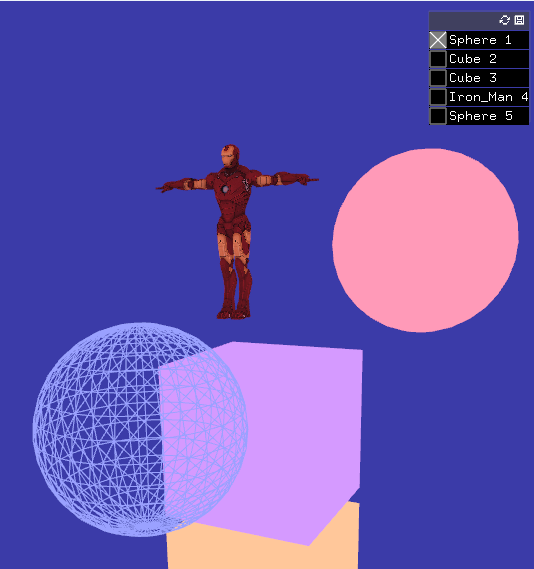
\includegraphics[width=12cm]{fig/WireframeSelection.png}
	\caption{La selection est en wireframe}
	\label{fig:test}
\end{figure}

\newpage

Les transformation géométriques peuvent être appliquées en même temps à toutes les entités sélectionnées, en appliquant une matrice de transformation à chacun d'entre eux en même temps. Cette matrice est créée à partir de "sliders", de translation, de rotation et de taille.

\begin{figure}[h]
	\centering
	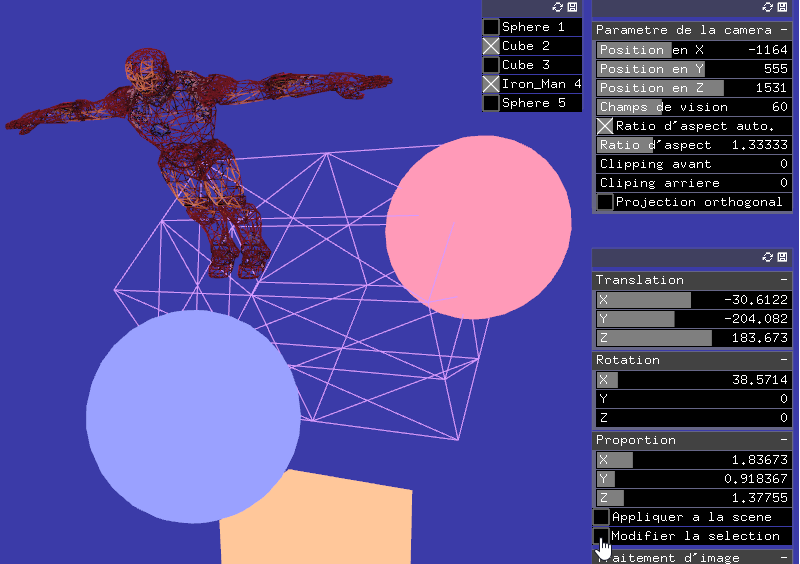
\includegraphics[width=18cm]{fig/transformationSelection.png}
	\caption{Chaque entité de la selection reçoit la transformation}
	\label{fig:test}
\end{figure}

\subsection{Coordonnées non-cartésiennes}
Non-implémenté

\subsection{Historique}
Non-implémenté

\section{Géométrie}
\subsection{Particules}
Non-implémenté

\subsection{Primitives}

Dans notre application, il est possible de créer à partir d'algorithmes seulement plusieurs primitives en 3D. Ces primitives sont le cube, la sphère et le cône. Chaque primitive peut être créée directement avec une position et taille choisie par l'utilisateur, mais ces attributs pourront bien évidemment être modifiées par la suite (voir la section 4.3.3 sur la sélection multiple.).

On ne peut pas créer les primitives avec une rotation dès le départ, car ce n'est pas pertinent de donner une rotation à un objet comme un cône, quand il n'y aucun moyen de savoir quel est son orientation "sans rotation" avant d'en avoir créé un de toute façon. Il faut leur donner la rotation voulue après les avoir créées.

On peut aussi choisir une couleur par primitive, dans l'espace de couleur HSB.

\begin{figure}[h]
	\centering
	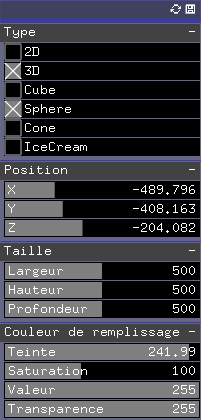
\includegraphics[width=6cm]{fig/creationPrimitive.png}
	\caption{Options de création d'une primitive}
	\label{fig:test}
\end{figure}

\subsection{Modèle}

Il est possible pour un utilisateur d'importer un modèle choisit sur son ordinateur. Les modèles supportés sont ceux qui ont un des formats suivants:

\begin{list}{}{}
	\item 3DS \tab ASE \tab DXF \tab HMP \tab MD2 \tab MD3
	\item MD5 \tab MDC \tab MDL \tab NFF \tab PLY \tab STL 
	\item X \tab LWO \tab OBJ \tab SMD \tab Collada \tab LWO
	\item Ogre XML \tab partly LWS
\end{list}

\begin{figure}[h]
	\centering
	\includegraphics[width=6cm]{fig/importerModele.png}
	\caption{Bouton pour importer un modèle}
	\label{fig:test}
\end{figure}

Si le modèle est dans un répertoire avec ses textures dans le bon chemin relatif, celles-ci seront automatiquement chargées et appliquées. De plus, si l'importation du modèle échoue pour une quelconque raison, un message sera affiché à l'utilisateur pour l'informer.

Un modèle peut être sélectionné comme une primitive, sera affecté par le mode "Wireframe", et sera modifié si on applique une matrice de transformation pendant qu'il est sélectionné.

\subsection{Texture}
Implémenté

\subsection{Géométrie procédurale}
Non-implémenté

\pagebreak
\section{Caméra}
\subsection{Propriétés de caméra}
Helllo there????

\begin{figure}[h]
	\centering
	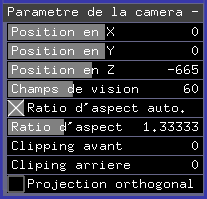
\includegraphics[width=5cm]{fig/proprieteCamera.png}
	\caption{Propriété de la caméra dans l'interface}
	\label{fig:test}
\end{figure}

\subsection{Mode de projection}
Le changement de mode de projection de perspective à orthogonale a été implémenté dans l'application. L'essentiel du travail se fait dans la méthode ccamera::changeMode(). Elle est appelé lorsqu'on appuit sur le bouton à cet effet dans l'interface graphique.

\begin{lstlisting}
	if (ortho.get()) {
		cam->enableOrtho();
	} else {
		cam->disableOrtho();
	}
\end{lstlisting}

\subsection{Caméra interactive}
La caméra interactive est implémenter dans l'application principalement à l'aide de la classe ofEasyCam de openFrameworks. Nous avons tout de même ajouter la possibilité de déplacer à l'aide des flèches du clavier, pour permettre de repositionner facilement la caméra. Il est aussi possible d'avancer à caméra à l'aide de pageUp/Down. L'essentiel du code se trouve au début de «ccamera::update()».

\begin{lstlisting}
	float dist = speed * dt;
	float dx = 0;
	float dy = 0;
	float dz = 0;
	
	dx = 0;
	if (isCameraMoveLeft)
		dx += dist;
	if (isCameraMoveRight)
		dx -= dist;
	cam->truck(-dx);
	posX.set(round(-cam->getX()));
	
	dy = 0;
	if (isCameraMoveUp)
		dy -= dist;
	if (isCameraMoveDown)
		dy += dist;
	cam->boom(-dy);
	posY.set(round(cam->getY()));
	
	dz = 0;
	if (isCameraMoveForward)
		dz -= dist;
	if (isCameraMoveBackward)
		dz += dist;
	cam->dolly(dz);
	posZ.set(round(cam->getZ()));
\end{lstlisting}

\subsection{Caméra multiple}
Non-implémenté

\subsection{Caméra animée}
Non-implémenté

\chapter{Ressources}
\label{s:ressources}

Voici la liste des ressources externes que nous avons utilisées dans le cadre du projet
\begin{enumerate}
	\item Notes de cours et exemple d'infographie 
	\item Modèle 3D d'Iron man téléchargé sur le site TF3DM à l'adresse:  \url{http://tf3dm.com/3d-model/iron-man-36822.html}
	\item Modèle d'Alduin téléchargé sur le site TF3M à l'adresse: 
	\url{http://tf3dm.com/3d-model/alduin-15997.html}
	\item Code pour produire une boite de dialogue trouvé sur le site Microsoft Developer Network à l'adresse: \url{https://msdn.microsoft.com/en-us/library/windows/desktop/bb776913(v=vs.85).aspx?f=255#\&MSPPError=-2147217396}
	\item ofxGui
	\item ofxOpenCv
	\item ofxAssimpModelLoader
\end{enumerate}
\chapter*{Présentation}
\label{s:presentation}

\appendix
\input{tex/appendix}

\end{document}
